\documentclass[oneside]{article}

% Font
\usepackage[T1]{fontenc}
\usepackage[utf8]{inputenc}
\usepackage{lmodern}

% For symbols
\usepackage{pifont}
\newcommand{\xmark}{\ding{53}} % x

% For tables
\usepackage{adjustbox}
\usepackage{multirow}
\usepackage{color, colortbl}
\definecolor{Gray}{gray}{0.95}
\usepackage{hhline}

% For identing the table at the right place
\usepackage{float}

% For left spacing
\usepackage{scrextend}

% For images
\usepackage{graphicx}
\usepackage[labelfont=bf]{caption}
\graphicspath{ {./images/} }

% links
\usepackage{hyperref}

% writting code
\usepackage{listings}
\definecolor{dkgreen}{rgb}{0,0.6,0}
\definecolor{gray}{rgb}{0.5,0.5,0.5}
\definecolor{mauve}{rgb}{0.58,0,0.82}
\lstset{frame=tb,
  language=python,
  aboveskip=3mm,
  belowskip=3mm,
  showstringspaces=false,
  columns=flexible,
  basicstyle={\small\ttfamily},
  numbers=none,
  numberstyle=\tiny\color{gray},
  keywordstyle=\color{blue},
  commentstyle=\color{dkgreen},
  stringstyle=\color{mauve},
  breaklines=true,
  breakatwhitespace=true,
  tabsize=3
}

% for shorter paragraph spaces
\setlength{\parindent}{1ex}
\setlength{\parskip}{0.5ex}
% for first paragraphs
\newcommand*\fpar{\hspace{1ex}}

\title{Project - Phase 8 Report}
\author{Group 14 \\
Tiago Carvalho fc51034 \\
Diogo Lopes fc51058 \\
Miguel Saldanha fc51072 \\
João Roque fc51080 \\
João Afonso fc51111 \\
}
\date{16/05/2021}

% The report is expected to:
  % Document the actual contributions in the various phases
  % Discuss the options taken throughout the project
  % Use diagrams and tables that summarize the ideas and results
  % Point future improvements

%  The report should not:
  % Explain concepts
  % Detail used frameworks, methodologies …
  % Use generic images or diagrams

\begin{document}
\maketitle

\section{Motivation}
\label{sec:motivation}
\fpar The idea for our project emerged when we were wondering how cool it would be to have an API that could help us decide which shows to watch next based on our personal taste. We figured that such a service could be developed with relative ease if users marked shows as viewed and/or liked.
\par Because users can watch more than just movies, for example animes, we wanted to use more than one dataset. Both animes and movies can have a lot in common not only with each other but also with books, so we also decided to use a book dataset. Using data from multiple datasets would give us a more realistic experience when it comes to cloud-native applications development, since these applications use data from so many sources.
\par With three datasets, we aimed to be able to effortlessly search through any of them. We wanted users to be able to mark movies, animes or books as seen or liked, and get suggestions of what to see next. Since the datasets have very similar categories among them, suggesting books mixed with movies and animes would be a possibility that we thought would add value to our application.
\par Our idea to implement the suggestion mechanism was to base these suggestions on the user's likes and views, which would indicate to us which categories the user prefers, and, therefore, allow us to suggest good movies, animes or books to the user.
\par We called our API “Seen”, since users can see movies, animes and books and then get suggestions based on their profile, on what they have seen.

\section{Dataset characterization}
\label{sec:dataset}
  \subsection{Dataset 1 — IMDB}
  \label{sec:movies}
  \fpar This dataset provides a lot of information about movies and shows that can be seen in \href{https://www.imdb.com}{IMDB}.
  \par We downloaded the dataset (updated one year ago) from the \href{https://www.kaggle.com/ashirwadsangwan/imdb-dataset}{Kaggle} website.
  \par From the whole dataset, these are the columns that were important to us:
  \begin{table}[H]
    \centering
    \begin{tabular}{l|l}
      Columns & Example                     \\ \hline
      id      & 606e2683b3fff1da8a207ae9    \\
      name    & The Arrival of a Train      \\
      category& [Action,Documentary,Short]  \\
      rating  & 7.4                         \\
      type    & short
    \end{tabular}
    \caption{Movie example in our database}
    \label{table:movie}
  \end{table}

  \subsection{Dataset 2 — MyAnimeList}
  \label{sec:animes}
  \fpar The second dataset, regarding the \href{https://myanimelist.net/}{MyAnimeList} website, was obtained from \href{https://www.kaggle.com/azathoth42/myanimelist}{Kaggle}.
  \par This dataset not only has a lot of anime content, but also user information, but because we want to connect with the other datasets it doesn't make sense to use that data. We used the following columns:
  \begin{table}[H]
    \centering
    \begin{tabular}{l|l}
      Columns & Example                       \\ \hline
      id      & 606e252aebddc73ebfb15507      \\
      name    & Shakugan no Shana: Season II  \\
      category& [Action,Drama,Fantasy,Romance,School,Supernatural]  \\
      rating  & 7.72                          \\
      imageUrl& https://myanimelist.cdn-dena.com/images/anime/10/18669.jpg
    \end{tabular}
    \caption{Anime example in our database}
    \label{table:anime}
  \end{table}

  \subsection{Dataset 3 — GoodReads}
  \label{sec:books}
  \fpar At last, this dataset represents books from the \href{https://www.goodreads.com/}{GoodReads} website, also downloaded from \href{https://www.kaggle.com/meetnaren/goodreads-best-books}{Kaggle}.
  \par The columns that are meaningful for us to be able to use this dataset together with the animes and movies datasets are the following:
  \begin{table}[H]
    \centering
    \begin{tabular}{l|l}
      Columns & Example                       \\ \hline
      id      & 606e25ad5e927a606f534284      \\
      name    & Of Mice and Men               \\
      description & The compelling story of two outsiders [...]           \\
      category& [Classics,Fiction,Academic,School,Literature,Historical]  \\
      rating  & 7.7                           \\
      imageUrl& https://images.gr-assets.com/books/1511302904l/890.jpg
    \end{tabular}
    \caption{Book example in our database}
    \label{table:book}
  \end{table}

\section{Use cases}
\label{sec:cases}
\fpar We have 3 types of Users: an Admin, which is a logged-in user with special permissions, a Regular user, which is a logged-in user, and a not logged-in user that we call Any.
\begin{table}[H]
  \centering
  \begin{tabular}{c|c|l} 
    Services & User & Functionalities \\ \hline
    \multirow{11}{*}{ Normal }
      & \multirow{2}{*}{ Any } 
        & Sign in \\
      & & See Book, Show and Movie Library \\ \cline{2-3}
      & \multirow{7}{*}{ Regular } 
        & User Log in \\
      & & Set Book/Show/Movie as seen \\
      & & Set Book/Show/Movie as liked \\ 
      & & Ask for suggestions to read and/or watch \\ 
      & & Count how many views a specific Item has \\
      & & Count how many likes a specific Item has \\
      & & Top 10 Items with more likes \\ \cline{2-3}
    & \multirow{2}{*}{ Admin } 
        & Add Book/Show/Movie to Library \\
      & & Remove Book/Show/Movie from Library \\ \hline
    \multirow{2}{*}{ Spark }
      & \multirow{2}{*}{ Any }
        & See best Director in terms of rating* \\
      & & See which Actor has the most connections \\
  \end{tabular}
  \caption{Seen's Use cases\\
          \**at least with $10$ movies and $10.000$ reviews in each}
\end{table}

\section{API}
\label{sec:api}
\begin{table}[H]
  \centering
  \addtolength{\leftskip} {-20cm}
  \addtolength{\rightskip}{-20cm}
  \begin{adjustbox}{width=1.6\textwidth}
  \begin{tabular}{ c|l l l l|c|c|c|c|l }
    \rowcolor{Gray}
    User & \multicolumn{4}{c|}{Path} & get & post & put & del & description 
    \\ \hline
    & /lib & \multicolumn{3}{l|}{/\{page\}} &
    \xmark & & & &
    Returns a $page$ from the database
    \\
    \multirow{-2}{*}{Regular} & 
    \multicolumn{4}{l|}{/suggest} &
     & \xmark & & &
    List of suggestions to watch
    \\ \hhline{-|----|-|-|-|-|~} \rowcolor{Gray}
    Admin & /item & & & &
    & \xmark & & &
    Creates an item to add to the database
    \\ \hhline{-|----|-|-|-|-|~}
    Any &
    /item & /\{type\} & /\{id\} & &
    \xmark & & & \xmark &
    Gets/Deletes item with specific $id$ and $type$ 
    \\ \hhline{-|----|-|-|-|-|~} \rowcolor{Gray}
    & /item & /\{type\} & /\{id\} & /seen &
    & & \xmark & &
    Marks item as seen
    \\ \rowcolor{Gray}
    \multirow{-2}{*}{Regular}
    & /item & /\{type\} & /\{id\} & /like &
    & & \xmark & &
    Marks item as liked
    \\ \hhline{-|----|-|-|-|-|~}
    & /item & /\{type\} & /\{id\} & /views &
    \xmark & & & &
    Returns Item's number of views
    \\
    & /item & /\{type\} & /\{id\} & /likes &
    \xmark & & & &
    Returns Item's number of likes
    \\ 
    & /getTopTen & /\{type\} &  &  &
    \xmark & & & &
    Returns top ten most liked Items with $type$
    \\ 
    & \multicolumn{4}{l|}{/user} &
    & \xmark & & &
    Creates User
    \\
    \multirow{-5}{*}{Any} 
    & /user & \multicolumn{3}{l|}{/login} &
    \xmark & & & &
    Logs in
    \\ \hhline{-|----|-|-|-|-|~} \rowcolor{Gray}
    & /user & \multicolumn{3}{l|}{/logout} &
    \xmark & & & &
    Logs out
    \\ \rowcolor{Gray}
    \multirow{-2}{*}{Regular} 
    & /user & /search & \multicolumn{2}{l|}{/\{username\}} &
    \xmark & & & \xmark &
    Searches/Deletes User by username
    \\ \hhline{-|----|-|-|-|-|~}
    & \multicolumn{4}{l|}{} &
     & & & &
    Returns the Director with best rating with \\
    & \multicolumn{4}{l|}{\multirow{-2}{*}{/\{director\}}} &
    \multirow{-2}{*}{\xmark}
     & & & &
    at least $10$ movies with $10.000+$ reviews
    \\ 
    & \multicolumn{4}{l|}{} &
     & & & &
    Returns the Actor's name with \\
    \multirow{-4}{*}{Any} 
    & \multicolumn{4}{l|}{\multirow{-2}{*}{/actor}} &
    \multirow{-2}{*}{\xmark} & & & &
    movies with the biggest cast in total
  \end{tabular}
  \end{adjustbox}
  \caption{Seen's API table}
\end{table}

\section{Architecture (application and technical)}
\label{sec:architecture}
  \subsection{Diagram}
  \begin{figure}[H]
    \centering
    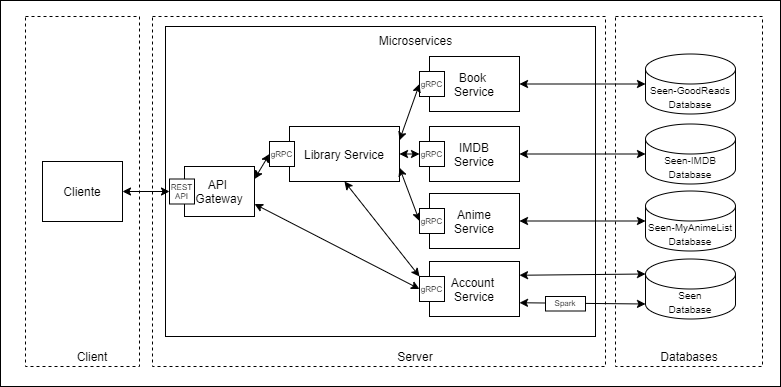
\includegraphics[width=\textwidth]{ CloudNativeAppArchitecture.png }
    \caption{Project's architecture.}
    \label{img:architecture}
  \end{figure}

  \subsection{Application}
    \subsubsection{Client}
    \fpar The Client should be able to access our API on his browser:
    \begin{center}
      \url{https://recommendations.sytes.net}
    \end{center}
    \par The Swagger provides a user interface to use and test our calls by adding "/ui" to the end of the url above.

    \subsubsection{Server}
    \fpar In total there are 7 different microservices working at the same time. Every single one of them runs on Google Cloud, inside the same cluster but in different dockers.
    \par Our reasoning was to have an entrance microservice, which would redirect the request to the microservice responsible for that type of request, for example when sending a request for a page in our library, the API Gateway receives that request and sends it to the Library Service, which is responsible for asking for books, movies and animes to the Book, IMDB and Anime Services, respectively, and then put them together in just one response, which is then sent to the API Gateway, to be shown to the Client.
    \par This API Gateway service also has the responsibility of transforming the REST requests from the Client to gRPC requests that are used internally, between Services.
    \par From the total of 7 microservices, 5 are responsible for the database connection, meaning that they are responsible for translating the request they receive into inserts, updates, removes or queries to the database. They are also responsible for translating responses from the database into responses that can be understood by the other microservices.

    \subsubsection{Databases}
    \fpar Every database has a service that has the responsibility to access and manage it. While 3 of the databases are hosted by \href{https://www.mongodb.com/}{MongoDB}, a NoSQL database, the last one is an SQL database hosted on an external server. This last database was initially hosted on Google Cloud, however we removed it from there, because it was costing us a lot of money.
    \par For the Books', Movies' and Animes' databases, we used a NoSQL database since we might have had to change the format of our documents, meaning that if we had an SQL database we would need to drop the entire database and repopulate it again every time we decided to change the schema. MongoDB provides a very easy and intuitive python implementation to work with, which was also a factor to consider when selecting the type of databases that we would be using.
    \par However, for the Users' database we used an SQL one, because we already knew what we wanted from the User, and we knew we would use structured data for it.

    \subsubsection{Spark}
    \fpar Later in the course of the project, we added the Spark microservice. This service receives the gRPC requests from the API Gateway service and then processes them, creating a job to send to Google Cloud where we have a Cluster with the sole purpose of running this type of jobs.

  \subsection{Technical}
  \fpar To implement the CI/CD pipeline, we created a trigger that when a commit is done on the deploy branch on git, the cloud build starts by running the yaml file. 
  \par First, it builds all the microservices, pushes them to the container registry, starts the Docker and runs the microservices. 
  \par After they are running, we start a test network using Docker, which is then tested (integration and unit tests), to assure that everything is alright and can be deployed on Kubernetes. If all the tests pass, the system is then deployed.

    \subsubsection{Server (Microservices)}
    % - plug ins
    %   - istio
    %   - auth0
    % - certificados e comunicações seguras
    \fpar TODO

    \subsubsection{Databases}
    \fpar Since the MongoDB already provides an API with secure channels we didn't need to make any changes to the connection, the transmitted data is secured, and we tested it by running Wireshark to sniff the packets and observing they are encrypted.
    \par To use a secure connection between the Service to handle the users' data we initialize a connection with certificates (SSL server certificate authority, SSL server certificate and an SSL client key) using the TLS cryptographic protocol designed to provide secure communications.

    \subsubsection{Spark}
    \fpar Having our jobs already on the cloud, the Spark Service (Spark Connector) has the responsibility of asking the Dataproc cluster for the result of the job that was requested, that will run it and send back the result.

\section{Implementation}
\label{sec:implementation}
\fpar We actually made 2 different implementations, one that runs locally and other that runs in the cloud.
\par We created a local version of our application for several reasons: we were more familiar with the development of local-running applications, running the application on the cloud costs money, and we can debug the app better when it is running locally which is important during development. When developing a feature, first we would put everything running locally, by running a script, and once the feature was running without issues on our machines, we would adapt it to run on the cloud.

  \subsection{Server (Microservices)}
    \subsubsection{Docker Compose}
    \fpar For the microservices deployment we use a docker-compose file, which defines each microservice. In this file, we define a microservice's name, a build stating that we are using a Dockerfile and where the context of the microservice is (its folder, with its required content). We also define the image, hostname and container for the microservice, for which we use the same name as the microservice's. Finally, we assign a port to the microservice, which is crucial for the application to behave properly.
    \par We do the steps stated before for every single microservice inside the docker-compose, but that's not all we have to do. Since the API Gateway service sends requests to the Spark Connector, Account and Library services, we add them as environment variables, meaning that when we run the python file defining the business logic of the service we can fetch the generated IP and then use it to connect to the services with gRPC channels. For the library we add all the services responsible for the databases, which are the Book, Imdb, Anime and Account services.

    \subsubsection{Dockers}
    \fpar To create a docker image for each microservice to be containerized we used dockerfiles. These files are really simple, they basically have everything they need in the folder they are in, and just make a new folder called service, and copy the current folder inside the newly created one. After copying, they run the installation of the requirements, using pip and the "requirements.txt" file. Then, the same port used on the docker-compose file before, is exposed to be accessible from outside this controller ambient/sandbox. Finally, the entry point is defined as the python file containing all the business logic of the microservice.

    \subsubsection{Protobuf Files}
    \fpar The protobuf files we created are the basis of our services communication between each other like we stated before.
    \par This files can be seen like interfaces that the services need to comply, so the recipient of the message processes it.
    \par We created an “utils” protobuf file, this file stores the interface of two messages, Success and Empty, and since they are repeatedly used we have them here to be ready to be imported. This file also stores an enumerated, with every Item type supported on this API: BOOK, SHOW and ANIME.
    \par Then the protobuf files are very straight forward, we define a protobuf service with the name of the actual Service that receives requests, and inside that protobuf service the functions that this Service supports.
    \par Those functions are also very simple, they consist in declaring a function that the Service has inside, with a message input and output, and the Service just has to comply with those restrictions, meaning that he receives a message of some type, and needs to “unpack” it and then “pack” it again to return as a response.
    \par Because we import the "utils" file, we then can use the Type (BOOK, SHOW or ANIME) that we declared inside other messages declarations. And use the “repeated” as a crucial part of our messages, since we usually want to send lists back and forth with our Item's content.
    \par To build the protobuf files into importable python files with all the necessary functions for communication we use a bash script, which compiles them and copies each one to the Services that use them.
      
    \subsection{Databases}
    \fpar Because we are using the free subscription of MongoBD, we can only have up to 512 Mb in each Cluster we create, this means we cannot fit inside one cluster all the data we have to store.
    \par To resolve this problem we created 4 different mongodb clusters, one for each Item type, and an extra one for the movie database, since the movie data set takes roughly 1Gb we had to split it in 2 halves.
    \par To upload our datasets, we used a script. The script connects to the database, then reads $100.000$ lines from the dataset, adapts each one with the relevant data to upload and then sends those $100.000$ items to the database. 
    \par Those adaptations are simple, using the csv package we can read both csv and tsv files row by row already split by columns. Then we transform the categories string into a list of strings, separating each category, facilitating queries. At last, we also strip the string from the white space at the beginning and at the end.
    \par About key duplicates we could have that problem using different databases, the generated key in one database could be the same as another one in another database, even if not likely it could happen. To resolve that problem we always use the type of the Item, with that type we choose which Service to send the request to, identifying the id and avoiding the “deletion” by omission of Items, because the first id found would be the one returned, omitting other results.
    \par For the movie database we also prepend (insert at the beginning) a database identification (“1” for the first half of items and “2” for the second one).
    \par For the user database we used another strategy and started an SQL database using SQLAlchemy to connect, using a secure channel with TLS.
    \par To maintain the same structure inside and outside the database we also created a python file named models, which has the correspondent classes to the tables inside the database, this way we can use those classes to fetch results already formatted. 

    \subsection{Spark}
    % TODO microserviço e implementação


\section{Evaluation and validation}
\label{sec:evaluation_and_validation}
\fpar To perform an evaluation on the system by load testing, we used three different technologies: Prometheus, Grafana and Locust. 
\par Prometheus is a monitoring system that retrieves data directly from the cluster as it is executing, while Grafana displays and amalgamates the data in a way that can be analyzed by the human eye (plots, etc.). 
\par To perform the load tests on itself, we used Locust, a load testing tool. 
\par All these tools were configured automatically with scripts to further automate the deployment of the system (see locust.sh and add\_plugins.sh).
\par To test our Spark implementation we used the interface inside the Google Cloud named Dataproc.

  \subsection{Evaluation}
  \label{sec:evaluation}
  \fpar We ran Locust, the tool to perform the load testing, in another cluster to avoid affecting the results. It was tested with up to 800 users, which at that point it was getting close to 100\% CPU usage, according to Grafana. 
  \par At the time, we were using weak machines (12 CPUs) as Google Cloud's free trial did not allow any higher than that. Every aspect of the system was being tested: getting entries, putting new entries, get pages from the database, get a recommendation (and even the login and logout which was later changed and so there is no need for load testing as it is handled by an exterior service, auth0). 
  \par We did load testing with 100 users, 500 users and 800 users which we assume to be a somewhat comfortable limit for the resources we have, it can go higher, but it could probably start running into performance problems after a certain point.
  \par For the Spark job we went to Google Cloud > Dataproc > Jobs, and observe the time taken running, and got 2 minutes and 5 seconds for the first one and 7 minutes and 37 seconds for the second.

  \subsection{Validation}
  \label{sec:validation}
  % dizer o que os resultamos que obtivemos querem dizer
  \fpar TODO

\section{Cost analysis}
\label{sec:cost}
% Analizar os custos, dizer porque não usámos SQL na goole cloud
\fpar TODO

\section{Discussion}
\label{sec:discussion}

  \subsection{Results}
  \label{sec:results}

  \subsection{Analysis}
  \label{sec:analysis}

\section{Conclusions}
\label{sec:conclusion}
% Foi possivel fazer o projeto em google cloud e ter uma api util e funcional bla bla bla

  \subsection{Contributions}
  \label{sec:contributions}

    \subsubsection{51034 - Tiago Carvalho}
    \subsubsection{51058 - Diogo Lopes}
    \subsubsection{51072 - Miguel Saldanha}
    \subsubsection{51080 - João Roque}
    \subsubsection{51111 - João Afonso}

  \subsection{Future alterations}
  \label{sec:alterations}

\section{Appendix}
\label{appendix}
% To store big images and reference them

\end{document}